\section{Technical Architecture}
\begin{figure}[H]
    \centering
    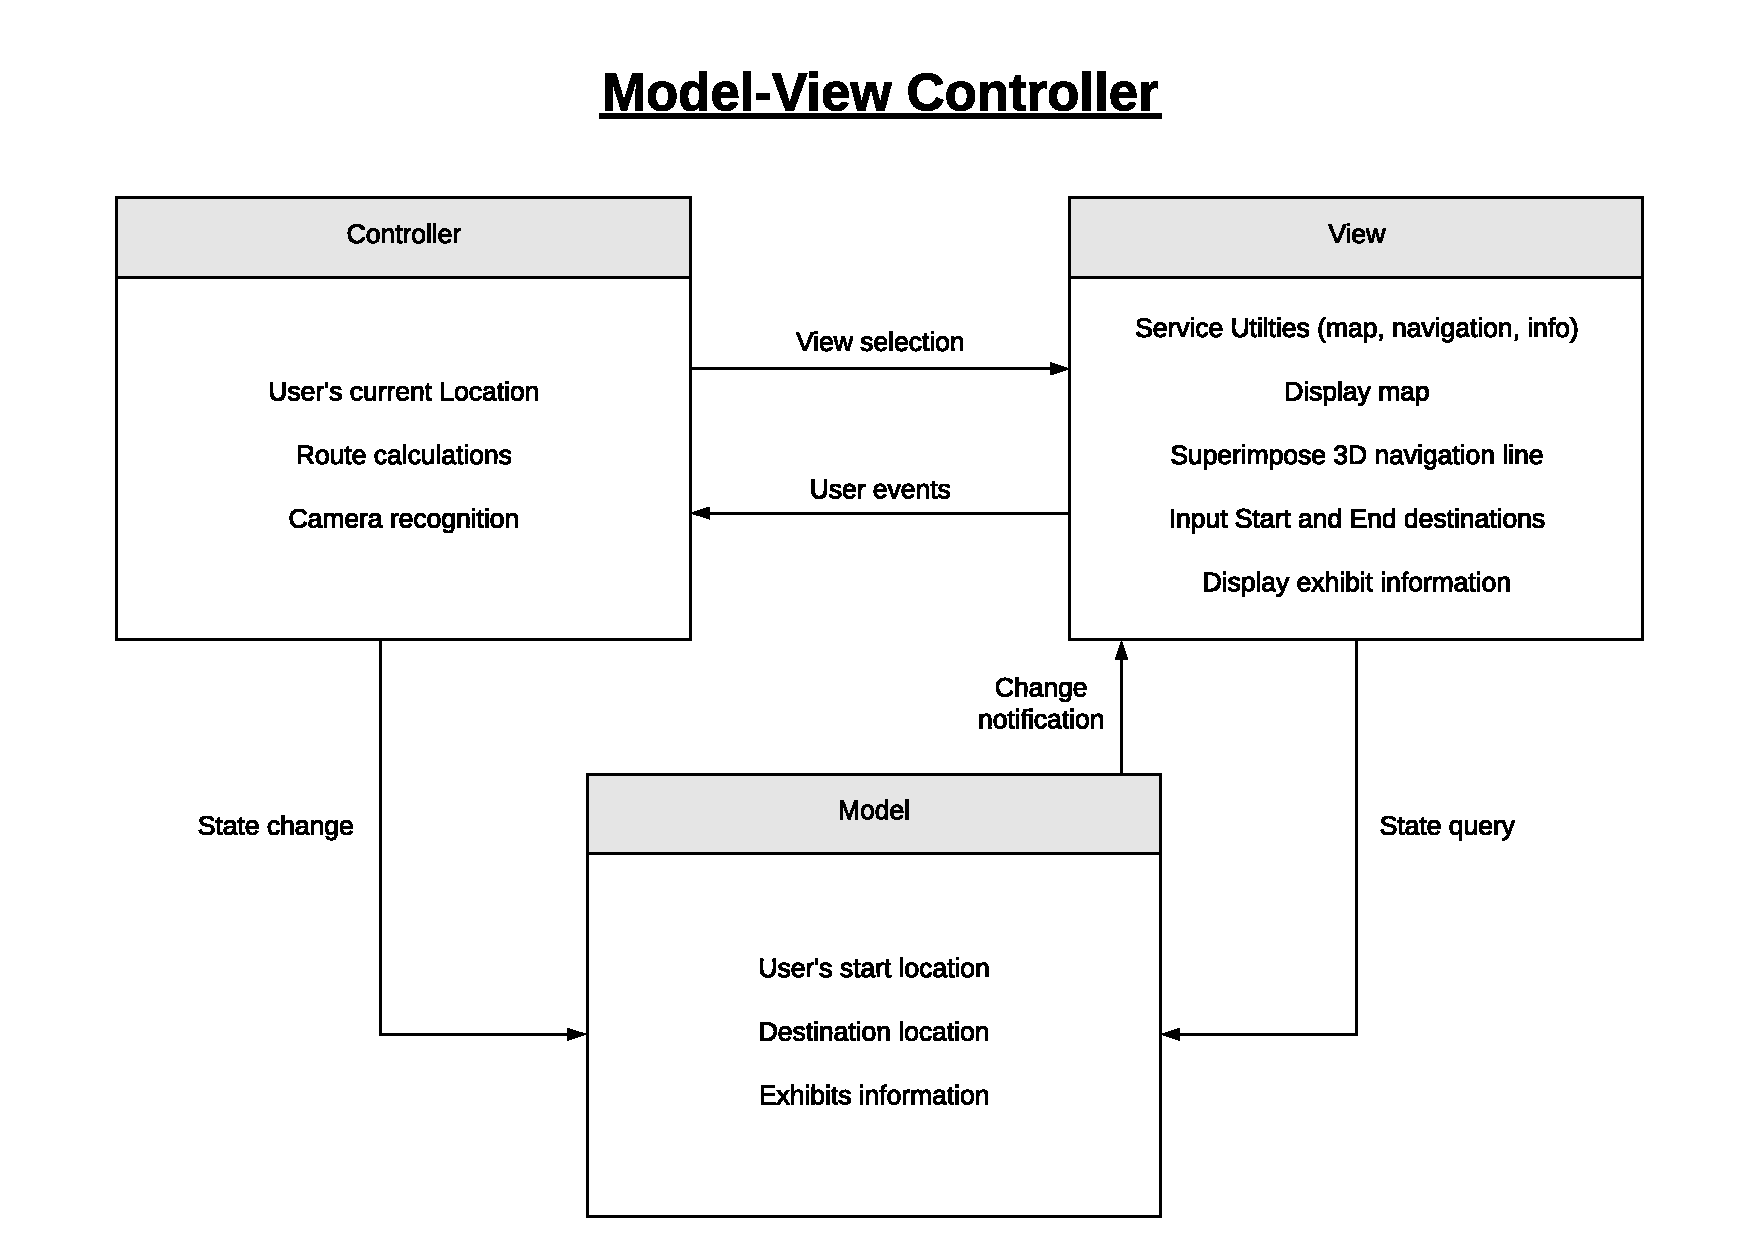
\includegraphics[width=\textwidth]
    {technicalarchitecture/mvc.pdf}
    \caption{MVC}
    \label{fig:technicalArchitecture}
\end{figure}

As a user-based application, a robust and reliable technical foundation is necessary in order for it to work successfully. It was quickly agreed upon that, the Model-View Controller (MVC) architecture (Figure~\ref{fig:technicalArchitecture}) would be the most relevant to creating the optimal version of the application. 

\subsection{Model}
The model of the MVC is the core component of an application. Data is stored and manipulated in this case, the users location, destination, and information held by the exhibit. These were to be manifested as a hard-coded location within a virtual geo-space to simulate the venue, and strings together data regarding the destination.

\subsection{View \& Controller}
Android devices were the conclusion from prototyping as the platforms to develop for. The construction of the front-end used Android Studio, and the back-end used ARCore, Java, and Kotlin. The front-end involved a login screen, a map screen, an information screen, and navigation screen; all were which controlled by the Java, and Kotlin code in the back-end.

\section{Models}
The following models are based on user interaction with the application.

\subsection{Use Case}
The use case diagram is crucial because it clarifies the lifecycle of a user during application runtime. Developing user-based applications like this becomes more manageable.

The use-case diagram (Figure~\ref{fig:model1}) deals with the two states that the user could be in; the lost state, and the exploration state.

The lost state is initialised by picking up the user's current location (once they have requested a destination) and calculating the shortest route between them, and their requested destination. This is finalised by collecting the user's current location, and displaying it to them via the superimposition of a 3D line in their camera view. From this step, the user just needs to follow the route until they arrive at their destination.

If the user considers another destination, or starts the application with no destination in mind. They have indirectly declared themselves to be in the exploration state. This state initialises itself by looking at the users past visits (if they have any) and current location to calculate recommendations. From this point on, once the user chooses a destination, the exploration state is identical to the lost state. The user follows the superimposed line and reaches their destination for the lifecycle to either begin again, or end.

\begin{figure}[H]
    \centering
    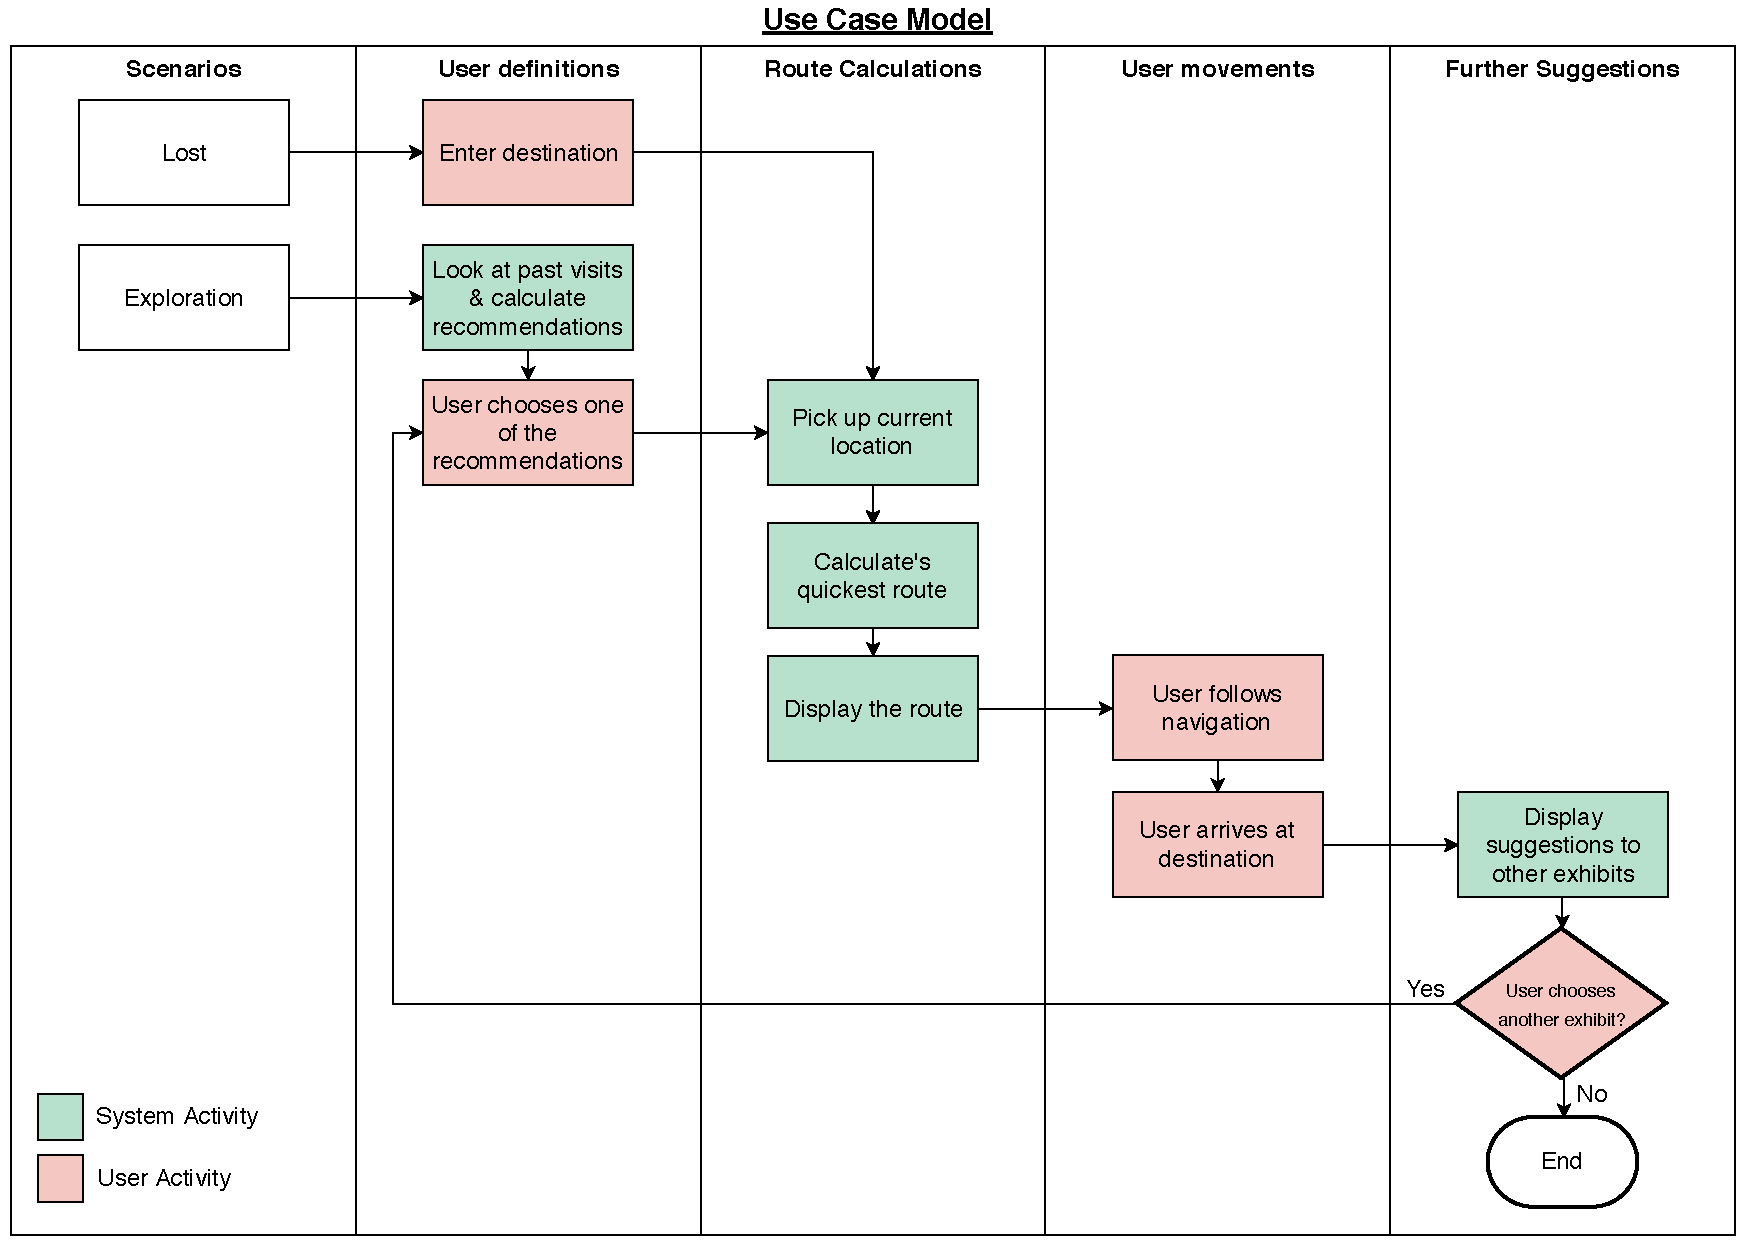
\includegraphics[width=\textwidth]
    {uml/use_case.pdf}
    \caption{Use case diagram}
    \label{fig:model1}
\end{figure}

\subsection{Activity}
The activity diagram (Figure~\ref{fig:model2}) distinguishes the details in two sections of the use case diagram, user definitions, and route calculations.

The route calculation process in the application is linear (Figure~\ref{fig:model2}). The user location is received from the GPS - distinguishing what venue the user is in. The building makeup is then requested from the server in order to make an analysis on the geospacial coordinates that the user will have to traverse. After the analysis is complete, the route between the user and destination requested in the user definition section can be calculated, and the route is superimposed.

User definitions that the activity diagram (Figure~\ref{fig:model2}) deals with are case specific to the exploration case. If the user would like to explore their venue, and they do not have one on the application; they are prompted to make an account so that the application can provide optimised recommendations. Inf they do, their previously visited locations can be used in presenting recommendations.

\newpage

\begin{figure}[H]
    \centering
    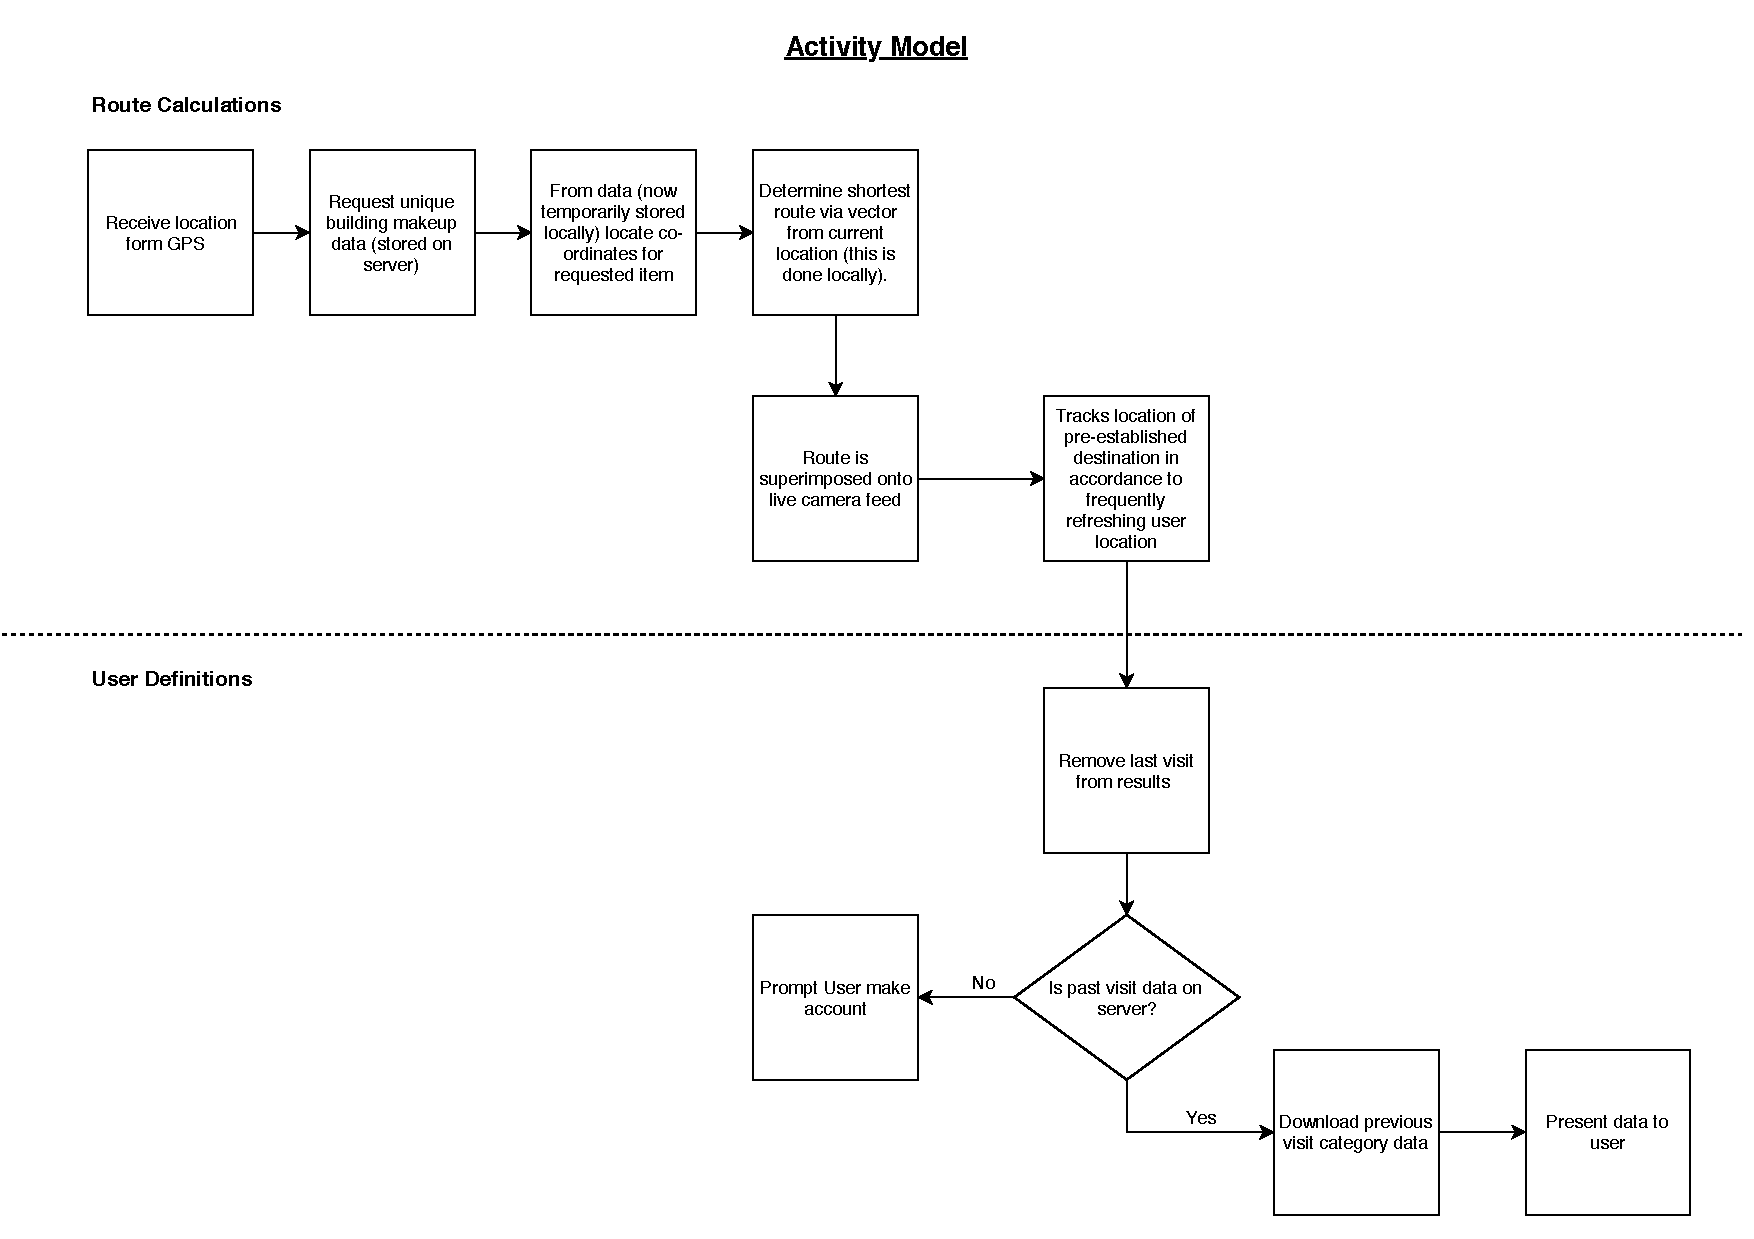
\includegraphics[angle=90, width=\textwidth]
    {uml/activity_diagram.pdf}
    \caption{Activity diagram}
    \label{fig:model2}
\end{figure}

\section{User Interface}
The project lends substantial importance to its user interface, and experience. As it will be used by people with a wide range of technical ability, the aim will be to make the app as simple as possible without having an impinging effect on any service the end product will feature. This prerequisite was clearly outlined in the surveying of museum visitors, and staff alike. The first mission was determining what interfaces, and experiences currently exists within the museum sector. Many museums employed simple interfaces but due to their mass-manufacturing, their design felt unoptimised with simple bare-bones media not beyond text and images. Furthermore, this design would fail to deliver anything more complex than texts and images.
  
The approach to the UI/UX prototyping was to create different interface mock ups, and exhibit them alongside existing solutions. An initial storyboard, and lo-fi prototypes was drawn up, and three potential interfaces (Figure~\ref{fig:prototype1}, ~\ref{fig:prototype2}, ~\ref{fig:prototype3}) were designed and shown to stakeholders. The feedback gained from the stakeholders was invaluable in the process as it allowed for the group to consider all aspects of the prototypes. It was decided that a final version of the application's user interface would be designed, implementing all the positive attributes, and combining it into one (Figure~\ref{fig:finaloverview}), whilst also considering the negative attributes.

\subsubsection{Prototype 1}
\begin{figure}[H]
    \centering
    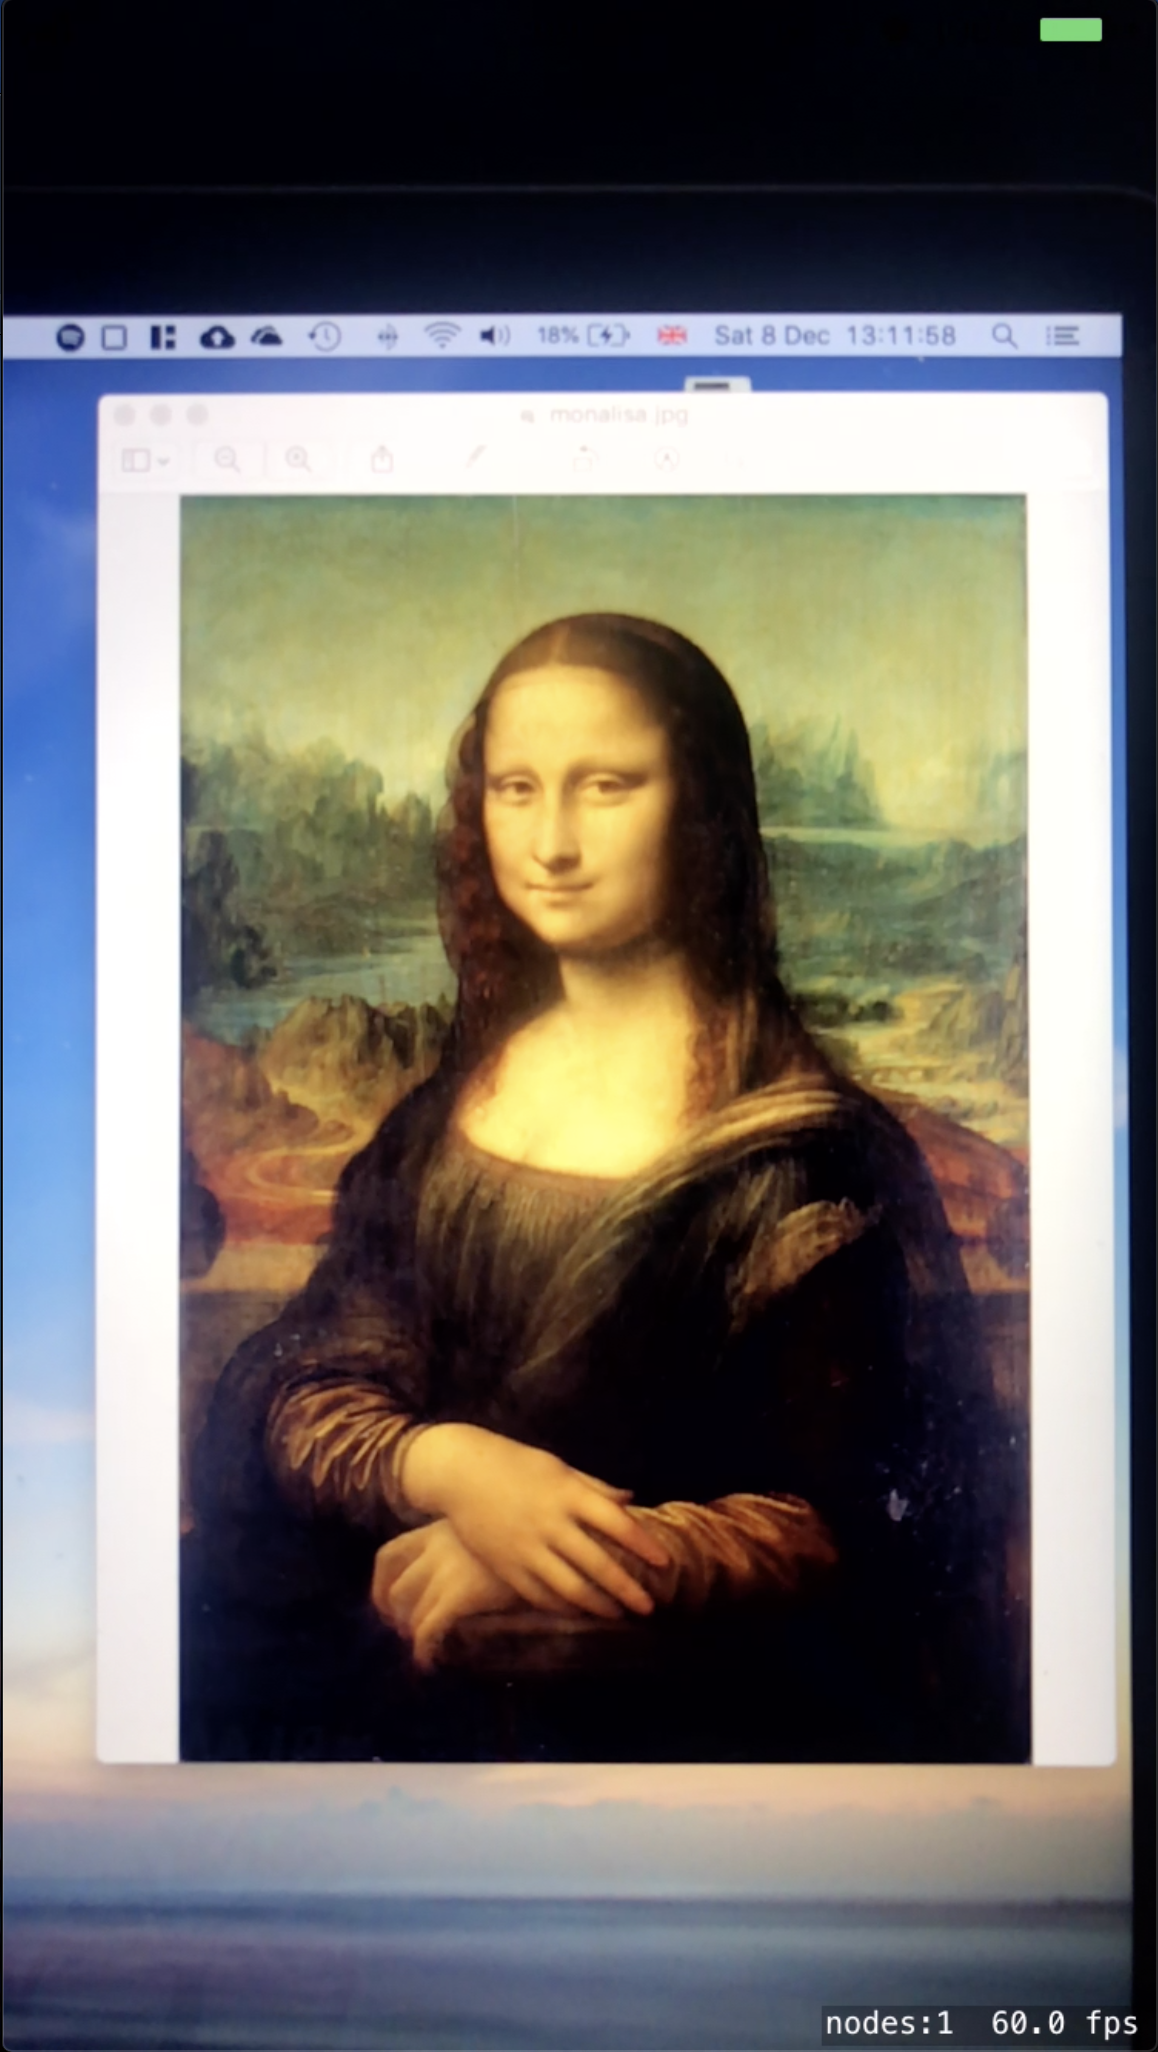
\includegraphics[width=\textwidth]
    {prototypes/ui/1.png}
    \caption{Overview of UI Prototype 1}
    \label{fig:prototype1}
\end{figure}

\subsubsection{Prototype 2}
\begin{figure}[H]
    \centering
    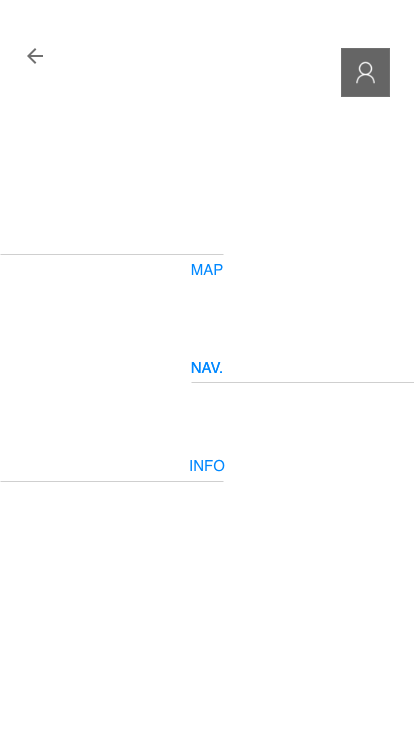
\includegraphics[width=\textwidth]
    {prototypes/ui/2.png}
    \caption{Overview of UI Prototype 2}
    \label{fig:prototype2}
\end{figure}

\subsubsection{Prototype 3}
\begin{figure}[H]
    \centering
    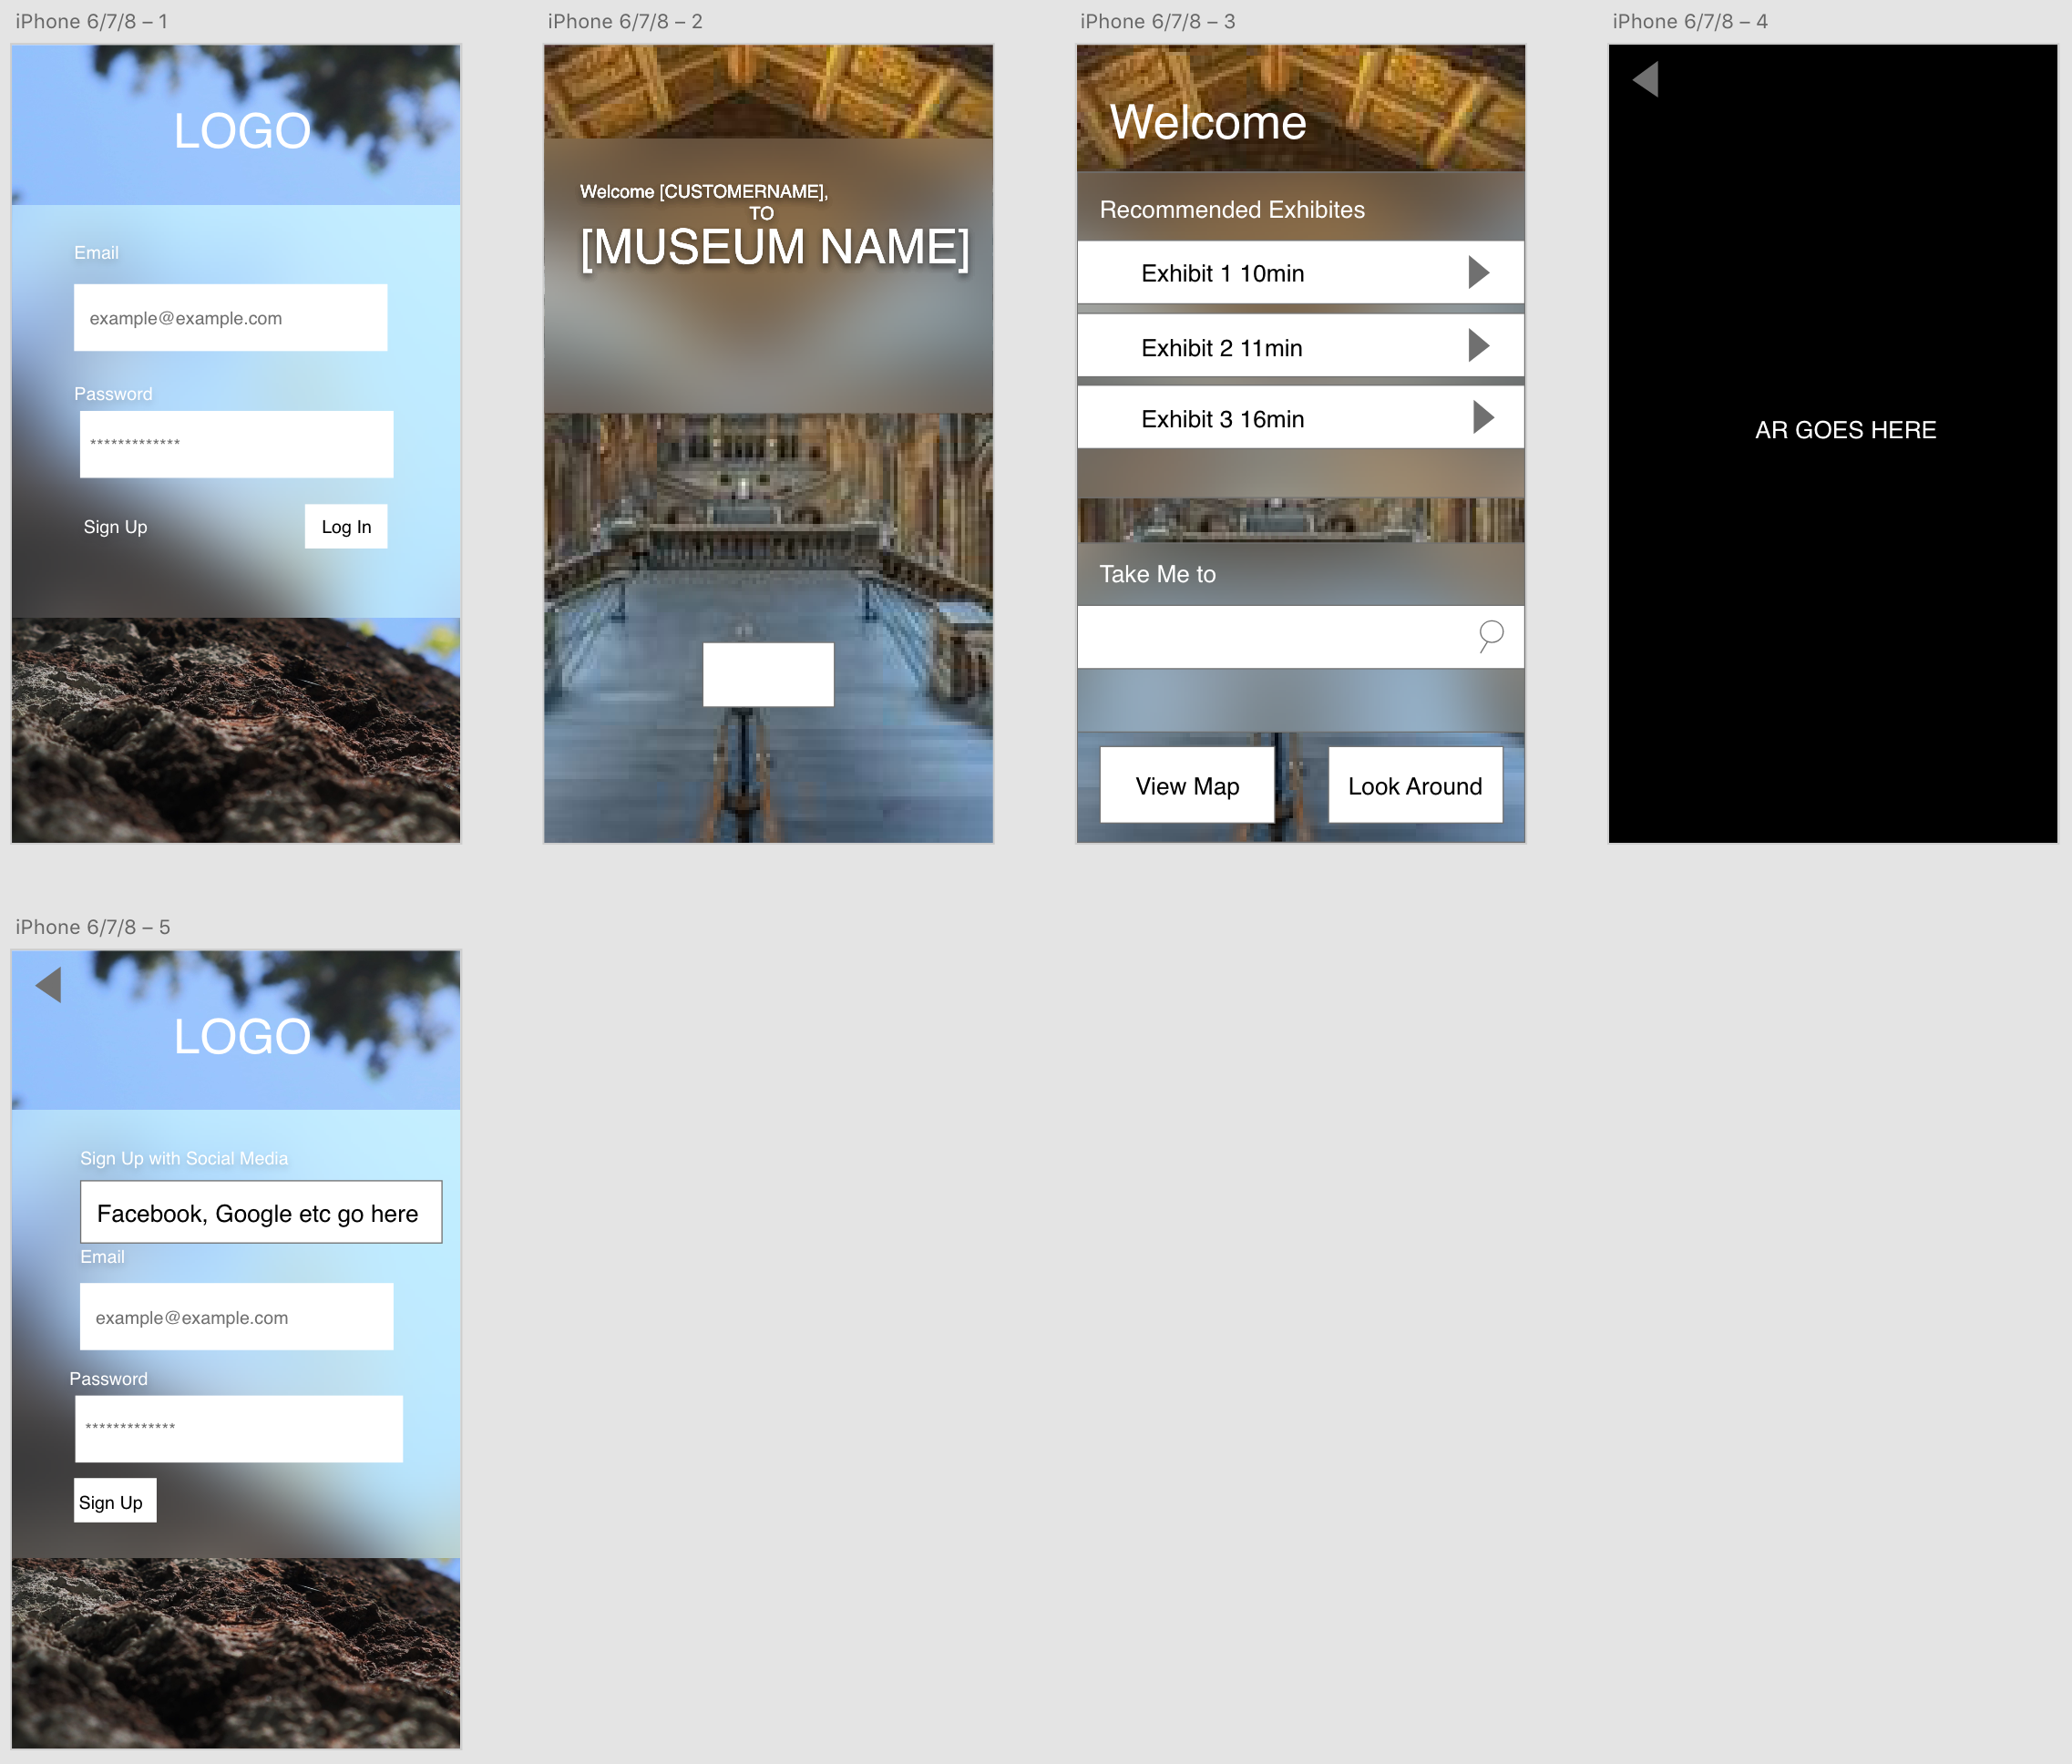
\includegraphics[width=\textwidth]
    {prototypes/ui/3.png}
    \caption{Overview of UI Prototype 3}
    \label{fig:prototype3}
\end{figure}

\newpage

\subsubsection{Final Prototype}
\begin{figure}[H]
    \centering
    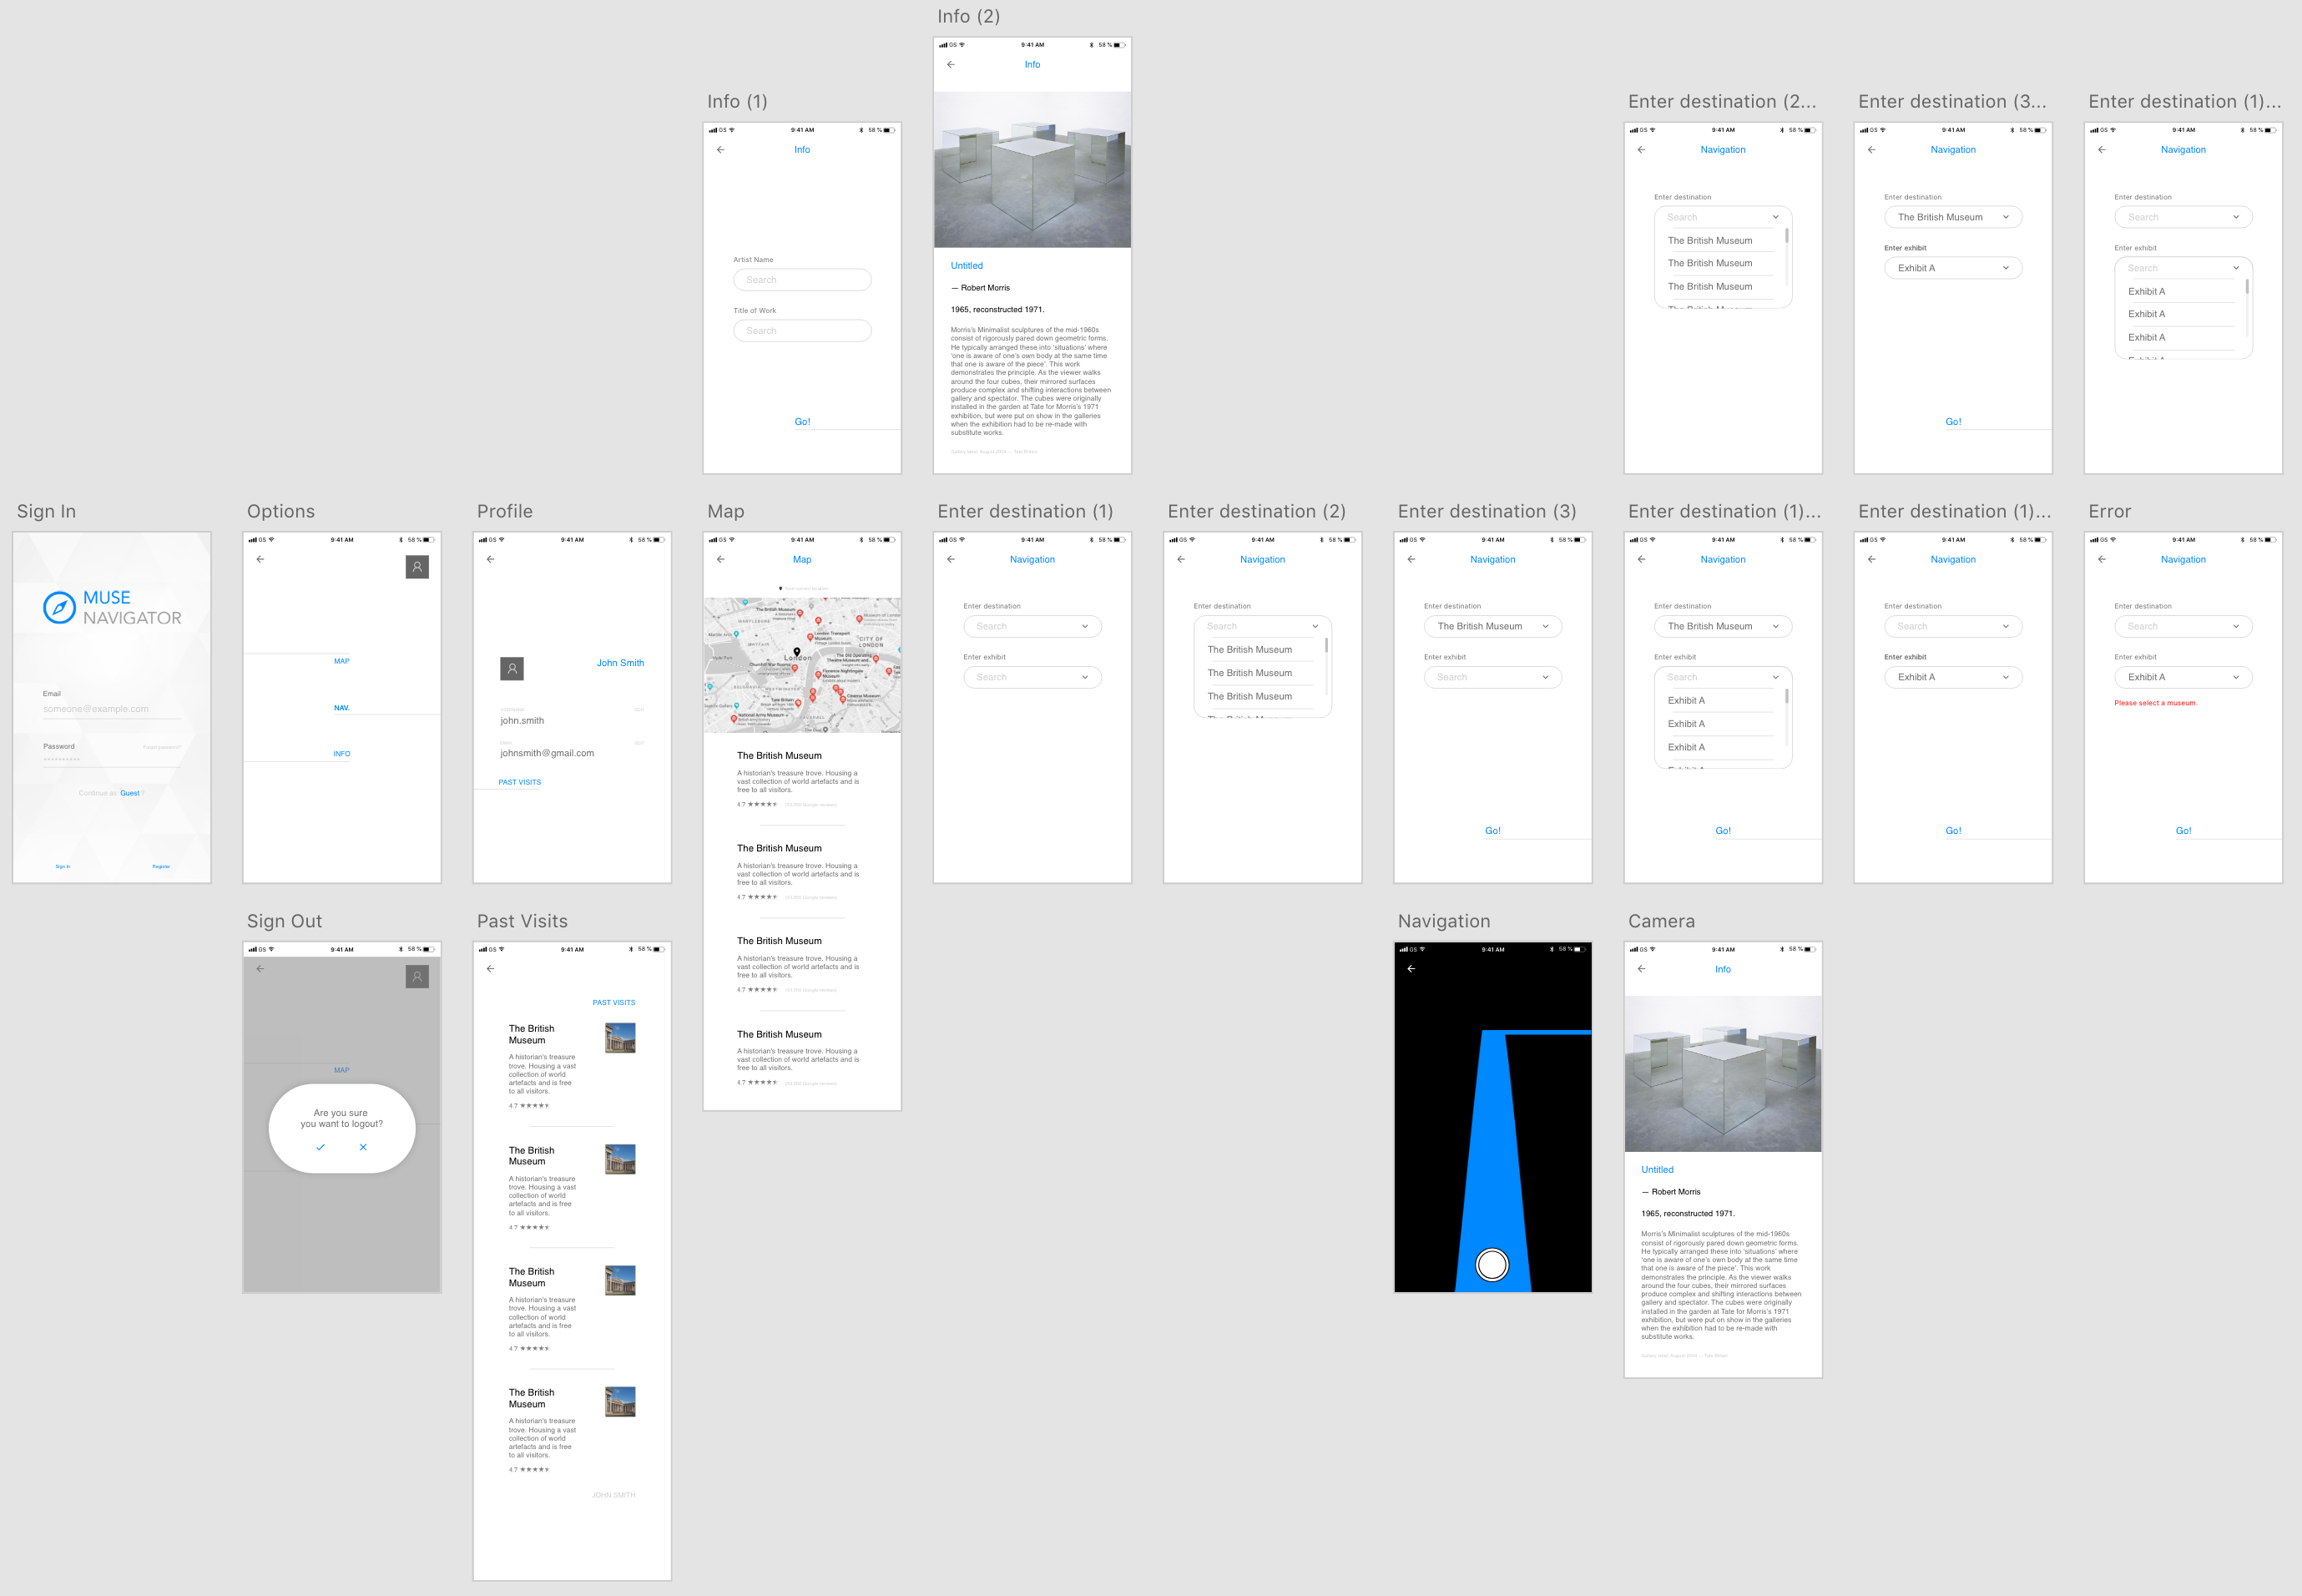
\includegraphics[angle=90, width=\textwidth]
    {prototypes/ui/final.png}
    \caption{Overview of final UI prototype}
    \label{fig:finaloverview}
\end{figure}

\newpage

\section{Accessibility}
The Web Accessibility Standard outlines key accessibility features for the group to consider. Some accessibility options would include features such as relating to mobility, colour perception, and literacy. Almost all museums have physical accessibility features managed, and features designed in the application have them incorporated in the design.

\begin{enumerate}
	\item \textbf{Screen Reading}: Users tend to rely on screen readers to help them interact with the app, including UI elements. This feature would allow the user to use the app without any difficulties since the layout is simple and straightforward. 

	\item \textbf{Scale}: Scale was used to allow for users to zoom, and resize elements in order to help those with visual impairments, particularly for images that include words. Font sizes across the application are not too small to ensure users of all ages can use it. Future iterations will include more scaling options through the app settings to allow for this.

	\item \textbf{Vision}: The text and UI in the app is designed to support high-contrast theme. Whilst colour is important, it must not be the only channel of communicating information. For instance, users who are colour blind would not be able to distinguish some colour status indicators from their surroundings.
    
\end{enumerate}